% This file is part of TenSing-Moers/Theaterskript2018.
%
% TenSing-Moers/Theaterskript2018 is free content: you can redistribute and/or
% modify it under the terms of the cc-by-nc-sa (Creative Commons
% Attribution-NonCommercial-ShareAlike) as released by the
% Creative Commons organisation, version 4.0.
%
% TenSing-Moers/Theaterskript2018 is distributed in the hope that it will be useful,
% but without any warranty.
%
% You should have received a copy of the cc-by-nc-sa-license along
% with this copy of TenSing-Moers/Theaterkskript2018. If not, see
% <https://creativecommons.org/licenses/by-nc-sa/4.0/legalcode>.
%
% Copyright TenSing Moers and all whose work and <3 went in this project.
\section{Alles (k)ein Traum?!}
\DisplayPersons
\DisplayRequisites
\ort{In \milamhh's Zimmer}

\StageDir{\miladh liegt im \bettd auf dem Boden und wälzt sich hin und her\dots}

\miladx{\direct{murmelt im Schlaf} Endlich\dots\ zu Hause\dots\ bin so\dots\ müde\dots\ \direct{schreckt hoch} \textbf{WAS?!} Wo?! \direct{setzt sich auf, sieht sich völlig verwirrt um} Oh man\dots\ Ich habe das doch jetzt nicht alles nur geträumt?!}

\StageDir{\mutterh kommt herein, setzt sich neben \miladh, schaut sie besorgt an.}

\mutterx{Mila? Bist du schon wach? Ist alles in Ordnung mit dir?}
\miladx{\direct{grinst} Was ist passiert?}
\mutterx{\alberthh hat dich gegen seine Weltreisemaschine geschubst, und dann bist du ohnmächtig geworden.}
\miladx{\direct{schlägt sich vor die Stirn} Oh nein! Und was ist mit der Aufführung?}
\mutterx{Die wurde verschoben.}
\miladx{Oh man\dots\ \direct{zu sich selbst} Ich muss das alles nur geträumt haben\dots}
\mutterx{Was hast du geträumt?}
\miladx{\direct{schnell} Nichts, nichts!}
\mutterx{Na gut. Weißt du schon, was du deiner Kusine Lucy schenken willst?}
\miladx{\direct{überrascht} Hm, vielleicht eine Karte für dieses Musical, von dem sie immer redet?}
\mutterx{Du meinst das mit dem Gospel-singenden Wissenschaftler, der ein Auto mit Avocado-Antrieb baut? Da wäre ich jetzt gar nicht drauf gekommen! Ich würde sogar was dazugeben\dots\ \direct{grinst} \dots\ aber auch nur, wenn du auch hingehst!}
\miladx{\direct{lächelt} Klar, total gerne! Ich würde gerne mal wieder was mit Lucy unternehmen! Und wer weiß, vielleicht lerne ich ja auch was über die chemischen Eigenschaften von Avocados\dots?}
\mutterx{\direct{legt \miladh die Hand auf die Stirn} Sicher, das es dir gut geht?}
\miladx{Klar! Sind \leonh und \lenah eigentlich schon wach?}

\StageDir{\leonh und \lenah kommen mit einem \raumschiffd auf die Bühne, lassen es durch die Luft fliegen und machen entsprechende Geräusche. Selbe Situation wie in Szene 2.}

\leonx{Mila, spielst du mit uns?}
\lenax{\direct{bettelt} Bitte, bitte!}
\mutterx{\direct{schmunzelt} Ich lasse euch drei dann mal alleine, okay? \direct{verlässt die Bühne}}
\lenax{\direct{trotzig, ruft \mutterh hinterher} Gar nicht okay! So spielt sie garantiert nicht mit uns.}
\miladx{Ach, warum denn nicht? Natürlich spiele ich was mit euch!}

\StageDir{\miladh steht auf, holt vier verschiedene \kugelnd hervor, setzt sich auf den Boden, und legt sie vor sich hin.}

\miladx{Zeig mal dein \raumschiffd, \leonh!}
\leonx{Aber sei vorsichtig! \leonh reicht ihr das \raumschiffd}
\miladx{\direct{ruhig} Ein schönes \raumschiffd hast du da. Sogar mit einem hochmodernen Avocadoantrieb! Und damit kann es zu vier ganz besonderen Planeten fliegen, am Rande unserer Galaxie! \direct{\glqq fliegt\grqq\ mit dem \raumschiffd um die \kugelnd herum.}}
\lenax{\direct{neugierig} Mit Aliens?}
\miladx{Mit Aliens. Ganz außergewöhnliche Aliens. Die sehen nämlich genauso aus wie wir, und reden auch wie wir. Aber wenn man genauer hinschaut, merkt man, dass sie eben doch keine Menschen sind, weil ihnen allen was fehlt. Auf diesem Planeten \direct{steuert eine/n der \kugelnd an} kann jeder machen, was er will, aber dafür\dots}
\lenax{\direct{eifrig} So wie in der Geschichte mit den Aliens, die ganz böse zueinander sind!}
\leonx{Ja! Und dann sind die plötzlich doch ganz nett.}
\miladx{\direct{neugierig} Was für eine Geschichte?}
\lenax{\direct{aufgeregt} Na, die in dem Buch, unter deinem Bett!}
\miladx{\direct{entsetzt} Ein Buch unter meinem Bett?! Meint ihr mein Tagebuch?? Habt ihr etwa in meinem Tagebuch gelesen?}
\leonx{\direct{beschämt, kleinlaut} Das Buch lag da so rum\dots\ Mir war langweilig, und du spielst ja nie mit uns. Und dann habe ich \lenah daraus vorgelesen\dots}
\lenax{\direct{begeistert} Genau! Und da stand was von vier Welten voller Aliens, zu denen du gereist bist! Hast du dir das für uns ausgedacht? Zum Spielen?}
\miladx{\direct{ungläubig} So einen Quatsch, das denkt ihr euch doch bloß wieder aus! \direct{wuschelt \leonh und \lenah durch die Haare} Ihr habt echt eine große Fantasie.}
\leonx{\direct{empört} Das haben wir uns nicht ausgedacht! Die Geschichte steht da wirklich! Die eine hatte so einen magischen Kuchen dabei, ich lieeebe Kuchen!}
\lenax{\direct{nickt bekräftigend, begeistert} Ja! Und Kekse und Bananen hast du geschenkt bekommen, weil du nur falsches Geld hattest, und die sind dir sogar bis auf's Klo gefolgt!}

\StageDir{\leonh und \lenah schauen sich an und kichern mit den Händen vor dem Mund.}

\miladx{\direct{entsetzt} Woher\dots\ Woher wisst ihr das alles?!}

\StageDir{\miladh springt auf, greift panisch nach dem Tagebuch, und blättert hektisch durch die letzten Seiten. Spot auf \miladh, wie sie mit fassungslosem Gesichtsausdruck und einem lauten Knall das Tagebuch fallen lässt.}

\begin{center}
\begin{Huge}
\textbf{Und Schluss!}
\end{Huge}

\vspace*{\fill}
\fbox{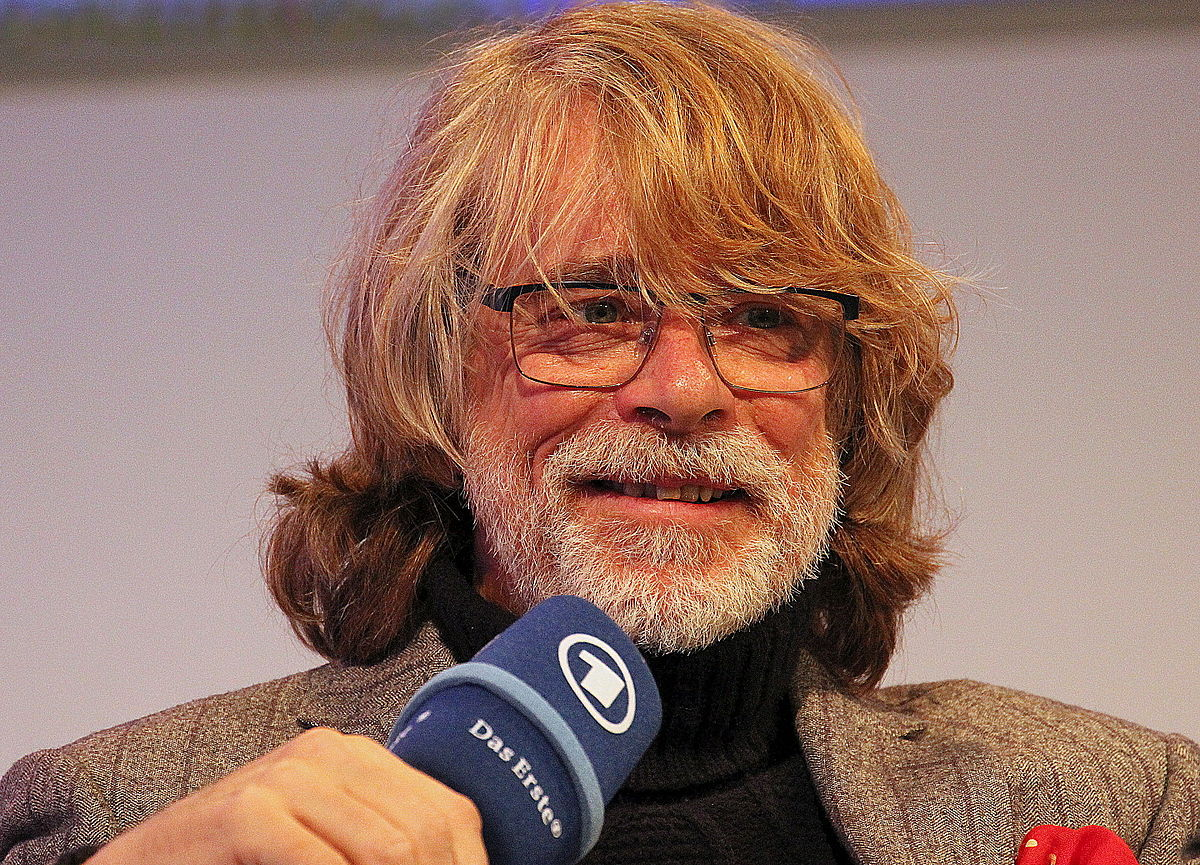
\includegraphics[scale=0.3]{res/1200px-Helge_Schneider_auf_der_Frankfurter_Buchmesse_2015.JPG}}
\end{center}